\documentclass[border=5pt]{standalone}
\usepackage{amsmath}
\usepackage{tikz}
\usetikzlibrary{positioning, fit, shapes, arrows}
\usetikzlibrary{chains}
\usetikzlibrary{calc}
\usetikzlibrary{decorations.pathmorphing}
\usetikzlibrary{decorations.pathreplacing}
\usetikzlibrary{shapes.multipart}
\begin{document}

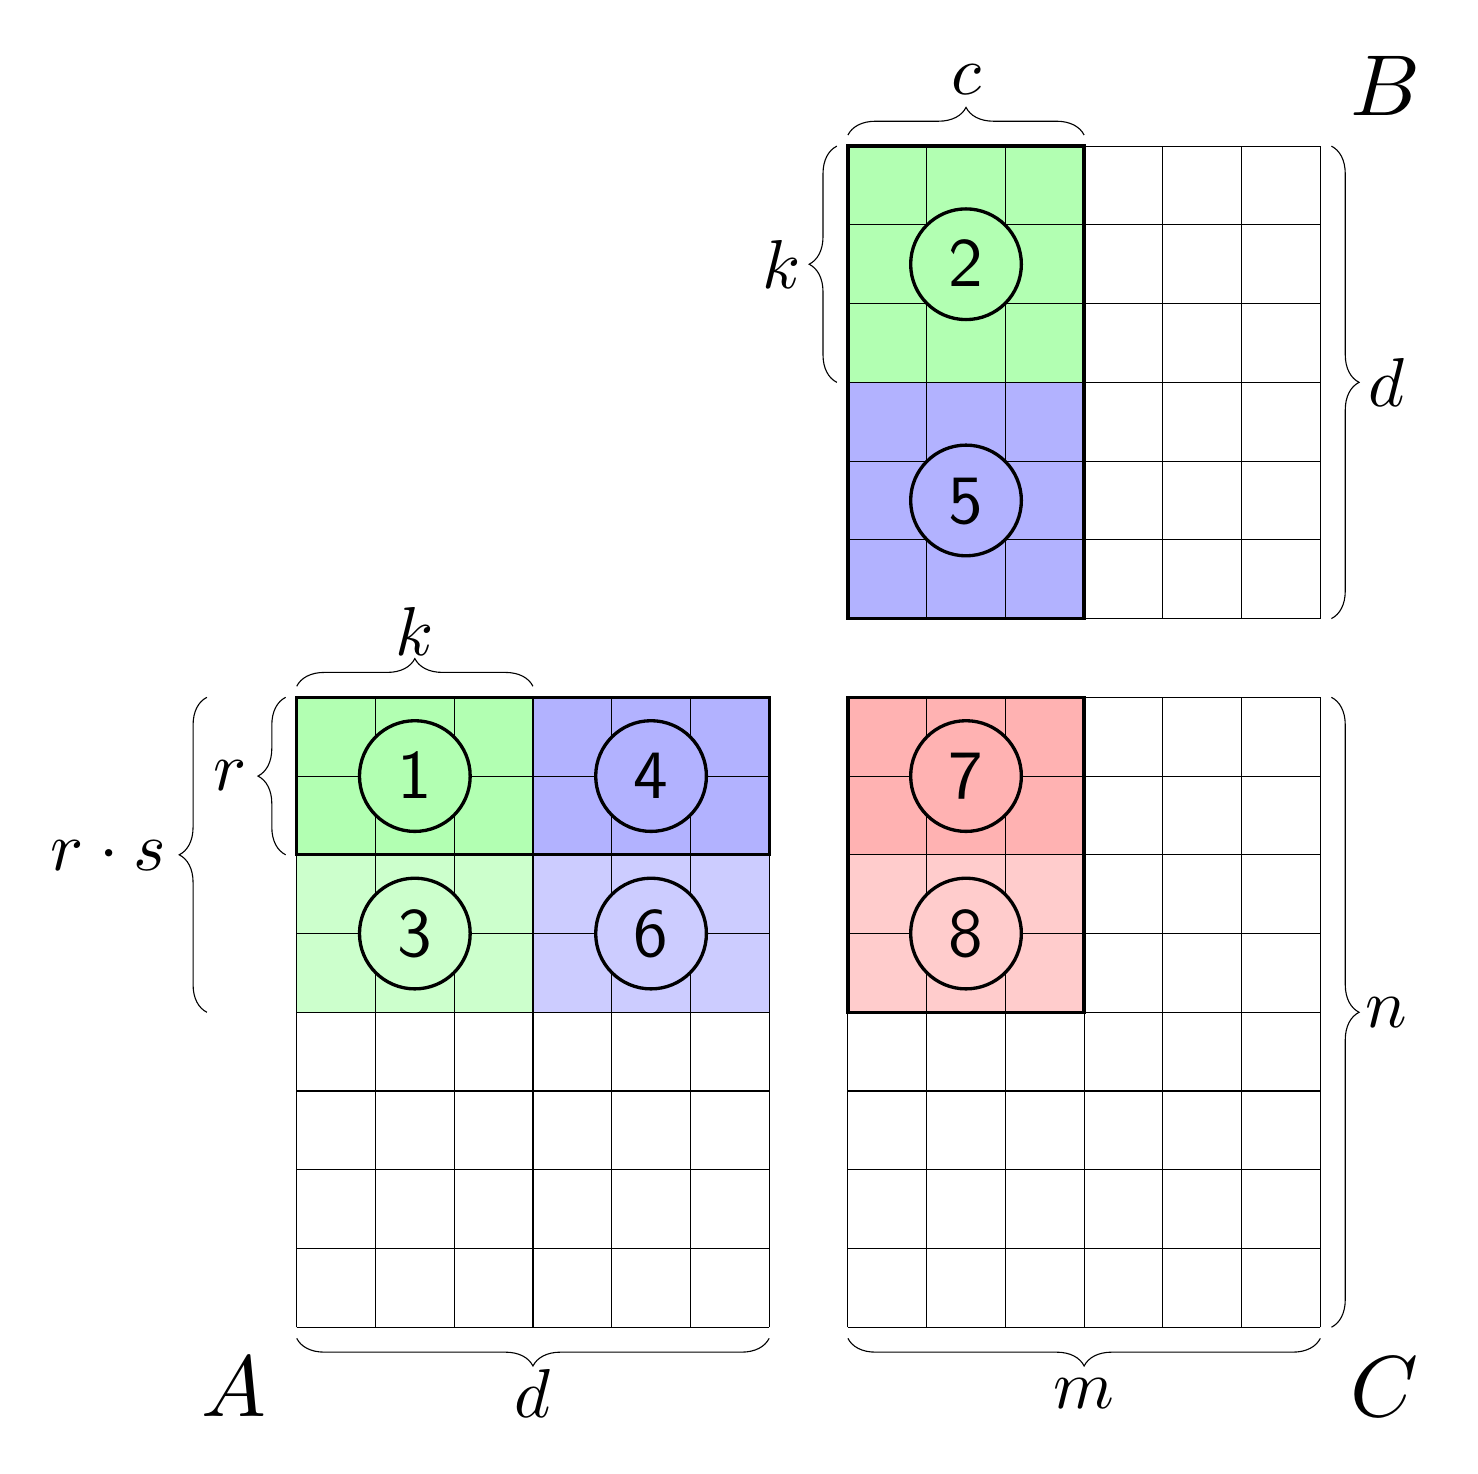
\begin{tikzpicture}[node distance=0.15 cm, font=\sffamily]

\newcommand{\scale}{2.5}
% A
\begin{scope}[xshift=-7cm]
  \fill[color=green!30] (0,6) rectangle (3,8);
  \fill[color=blue!30]  (3,6) rectangle (6,8);
  \fill[color=green!20] (0,4) rectangle (3,6);
  \fill[color=blue!20]  (3,4) rectangle (6,6);

  \draw[step=1cm, black, thin] (0,0) grid (6,8);

	\draw[very thick] (0,6) rectangle (6,8);

  \node[anchor=north east, scale=\scale*1.25] at (0,0) {$A$};

  \node[draw, circle, minimum size=40pt, line width=1.2, fill=green!30] (m) at (1.5,7) {};
  \node[scale=\scale] at (m.center) {1};
  \node[draw, circle, minimum size=40pt, line width=1.2, fill=blue!30] (m) at (4.5,7) {};
  \node[scale=\scale] at (m.center) {4};
  \node[draw, circle, minimum size=40pt, line width=1.2, fill=green!20] (m) at (1.5,5) {};
  \node[scale=\scale] at (m.center) {3};
  \node[draw, circle, minimum size=40pt, line width=1.2, fill=blue!20] (m) at (4.5,5) {};
  \node[scale=\scale] at (m.center) {6};

  \draw [decorate,decoration={brace,amplitude=10pt},yshift=4pt,xshift=0pt]
         (0,8) -- (3,8) node [black,midway,yshift=0.7cm,scale=\scale]  {$k$};

  \draw [decorate,decoration={brace,amplitude=10pt},xshift=-4pt,yshift=0pt]
         (0,6) -- (0,8) node [black,midway,xshift=-0.7cm,scale=\scale]  {$r$};

  \draw [decorate,decoration={brace,amplitude=10pt},xshift=-4pt,yshift=0pt]
         (-1,4) -- (-1,8) node [black,midway,xshift=-1.25cm,scale=\scale]  {$r\cdot s$};

  \draw [decorate,decoration={brace,mirror,amplitude=10pt},yshift=-4pt,xshift=0pt]
         (0,0) -- (6,0) node [black,midway,yshift=-0.7cm,scale=\scale]  {$d$};
\end{scope}

% B
\begin{scope}[yshift=9cm]
  \fill[color=green!30] (0,3) rectangle (3,6);
  \fill[color=blue!30]  (0,0) rectangle (3,3);

  \draw[step=1cm, black, thin] (0,0) grid (6,6);

	\draw[very thick] (0,0) rectangle (3,6);

  \node[anchor=south west, scale=\scale*1.25] at (6,6) {$B$};

  \node[draw, circle, minimum size=40pt, line width=1.2, fill=green!30] (m) at (1.5,4.5) {};
  \node[scale=\scale] at (m.center) {2};
  \node[draw, circle, minimum size=40pt, line width=1.2, fill=blue!30] (m) at (1.5,1.5) {};
  \node[scale=\scale] at (m.center) {5};

  \draw [decorate,decoration={brace,amplitude=10pt},yshift=4pt,xshift=0pt]
         (0,6) -- (3,6) node [black,midway,yshift=0.7cm,scale=\scale]  {$c$};

  \draw [decorate,decoration={brace,amplitude=10pt},xshift=-4pt,yshift=0pt]
         (0,3) -- (0,6) node [black,midway,xshift=-0.7cm,scale=\scale]  {$k$};

  \draw [decorate,decoration={brace,mirror,amplitude=10pt},xshift=4pt,xshift=0pt]
         (6,0) -- (6,6) node [black,midway,xshift=0.7cm,scale=\scale]  {$d$};
\end{scope}

% C
\begin{scope}[]
  \fill[color=red!30] (0,6) rectangle (3,8);
  \fill[color=red!20]  (0,4) rectangle (3,6);

  \draw[step=1cm, black, thin] (0,0) grid (6,8);

	\draw[very thick] (0,4) rectangle (3,8);

  \node[anchor=north west, scale=\scale*1.25] at (6,0) {$C$};

  \node[draw, circle, minimum size=40pt, line width=1.2, fill=red!30] (m) at (1.5,7) {};
  \node[scale=\scale] at (m.center) {7};
  \node[draw, circle, minimum size=40pt, line width=1.2, fill=red!20] (m) at (1.5,5) {};
  \node[scale=\scale] at (m.center) {8};

  \draw [decorate,decoration={brace,mirror,amplitude=10pt},xshift=4pt,xshift=0pt]
         (6,0) -- (6,8) node [black,midway,xshift=0.7cm,scale=\scale]  {$n$};

  \draw [decorate,decoration={brace,mirror,amplitude=10pt},yshift=-4pt,xshift=0pt]
         (0,0) -- (6,0) node [black,midway,yshift=-0.7cm,scale=\scale]  {$m$};
\end{scope}
    
\end{tikzpicture}
\end{document}
